% 
%
% (c) 2025 Autor, ETH Zürich
%
% !TEX root = linalg_I-II_summary.tex
% !TEX encoding = UTF-8
%

\section{Constructing New Vector Spaces Out of Old Ones}

\begin{proposition}{The Vector Space of Linear Functions}{vect_sp_lin_func}
	Let $V, W$ be two vector spaces over $K$. Then $\operatorname{Hom}(V, W)$ has the structure of a vector space over $K$, if we endow it with the following operations:
	\begin{itemize}
		\item[$\bullet$] $\forall \, T_1,T_2 \in \operatorname{Hom}(V, W), \; (T_1 + T_2)(v) := T_1(v) + T_2(v) \quad \forall \, v \in V$.
		\item[$\bullet$] $\forall \, T \in \operatorname{Hom}(V, W), \alpha \in K, \; (\alpha T)(v) := \alpha T(v) \quad \forall \, v \in V$.
	\end{itemize}
	The neutral element of $\operatorname{Hom}(V, W)$ is the map $0: V\to W, \quad v \mapsto 0$.
\end{proposition}

\begin{theorem}{The map $\Psi^{\mathcal{B}}_{\mathcal{C}}$}{map_psi}
	Let $V, W$ be finite dimensional vector spaces over $K$, $\mathcal{B} = (v_1 , \hdots , v_n)$ a basis for $V$, and $\mathcal{C} = (w_1, \hdots , w_n)$ a basis for $W$. Then the map
	\[
		\Psi^{\mathcal{B}}_{\mathcal{C}}: \operatorname{Hom}(V, W) \to M_{m \times n}(K)
	\]
	defined by
	\[
		T \mapsto [T]^{\mathcal{B}}_{\mathcal{C}} := \begin{pmatrix}
			\rule{0.5pt}{2ex} & & \rule{0.5pt}{2ex}\\
			[Tv_1]_{\mathcal{C}} & \hdots & [Tv_n]_{\mathcal{C}}\\
			\rule{0.5pt}{2ex} & & \rule{0.5pt}{2ex}\\
		\end{pmatrix}
	\]
	is a linear map and moreover an isomorphism.
\end{theorem}

\begin{corollary}{Dimesnion of $\operatorname{Hom}(V, W)$}{dim_hom}
	If $V, W$ are finite dimensional vector spaces then so is $\operatorname{Hom}(V, W)$ and $\dim \operatorname{Hom}(V, W) = \dim V \cdot \dim W$.
\end{corollary}

\subsubsection{Rings}
Recall that Rings have the same axioms as Fields except that we do \textbf{not} require that every non-zero element has an inverse.

\begin{definition}{Homomorphism of Rings}{homo_ring}
	Let $R, S$ be rings. A \textbf{homomorphism of rings} is a map $\varphi: R \to S$ s.t.:
	\begin{itemize}
		\item[$\bullet$] $\forall \, r_1,r_2 \in R : \, \varphi(r_1 + r_2) = \varphi(r_1) + \varphi(r_2)$.
		\item[$\bullet$] $\forall \, r_1,r_2 \in R: \, \varphi(r_1 \cdot r_2) = \varphi(r_1) \cdot \varphi(r_2)$
		\item[$\bullet$] $\varphi(1) = 1$.
		\item[$\bullet$] $\varphi(0) = 0$.
	\end{itemize}
\end{definition}

\begin{corollary}{$\Psi$ for an Endomorphism is an isomorphism of Rings}{endo_homo_ring}
	Let $V$ be a vector space over $K$. Then $\operatorname{End}(V) := \operatorname{Hom}(V, V)$ is a ring with a unity. This ring is, in general, not commutative. The multiplication (product) in $\operatorname{End}(V)$ is given by composition, i.e.,
	\[
		T_1 \cdot T_2 := T_1 \circ T_2 \qquad \forall \, T_1, T_2 \in \operatorname{Hom}(V,V).
	\]
	The unity is $id_V$. Moreover, if $V$ is finite dimensional and $\dim V = n$, and $\mathcal{B} = (v_1, \hdots , v_n)$ is a basis for $V$, then $\Psi^{\mathcal{B}}_{\mathcal{B}}: \operatorname{Hom}(V,V) \to M_{n \times n}(K)$ is an isomorphism of rings
\end{corollary}

\subsection{Dual Space}
An important special case of $\operatorname{Hom}(V,W)$ is when $W = K$.

\begin{definition}{Dual Space}{dual_sp}
	Let $V$ be a vector space over $K$. The \textbf{dual space} of $V$, is defined to be the vector space $V^* := \operatorname{Hom}(V,K)$. The elements of $V^*$ are linear maps $\ell :V \to K$, and are sometimes called \textbf{functionals} (on $V$).
\end{definition}

\begin{corollary}{Dimension of the Dual Space}{dim_dual_sp}
	Let $V$ be a finite dimensional vector space over $K$. Then $\dim V^* = \dim V$.
\end{corollary}

Let $V = K^n_{\text{col}}$. Then we can identify $V^*$ with $K^n_{\text{col}}$, as follows: If $\ell \in K^n_{\text{row}}$, then $\ell$ defines a functional $f_{\ell}:K^n_{\text{col}} \to K$ by $f_{\ell}(v) := \ell \cdot v \in K$. The map $D:K^n_{\text{row}} \to (K^n_{\text{col}})^*$ defined by $D(\ell) := f_{\ell}$ is a linear map and is an isomorphism.

Let $V$ be a finite dimensional vector space over $K$ and $\mathcal{B} = (v_1, \hdots , v_n)$ a basis for $V$. $\forall \, 1 \leq i \leq n$, define a functional $v_i^* \in V^*$, i.e., $v_i^*:V \to K$ linear map, as follows:
\[
	v_i^*(v_j) := \delta_{ij} = \begin{cases}
		1 & i = j\\
		0 & i \neq j
	\end{cases}.
\]
Since $v_1, \hdots , v_n$ form a basis for $V$, our definition determines uniquely a well-defined functional $v_i^*:V \to K$.

\begin{lemma}{\textcolor{red}{The Dual Basis}}{dual_base}
	The elements $v_1^*, \hdots , v_n^* \in V^*$ form a basis for $V^*$. This basis is called the \textbf{dual basis} to $\mathcal{B}$. We denote this basis by $\mathcal{B}^* = (v_1^*, \hdots , v_n^*)$.
	
	Moreover,
	\[
		\forall \, \ell  \in V^* : \, \ell = \sum_{i=1}^{n} \ell(v_i)\cdot v_i^*.
	\] 
\end{lemma}

\begin{proof}
	Let $\ell \in V^*$. We claim that 
	\begin{equation}
		\label{eq:dual_1}
		\ell = \sum_{i=1}^{n} \ell(v_i) \cdot v_i^*.
	\end{equation}
	Or in other words, we claim that
	\begin{equation}
		\label{eq:dual_2}
		\forall \, v \in V: \, \ell(v) = \sum_{i=1}^{n} \ell(v_i) \cdot v_i^*(v).
	\end{equation}
	Indeed, both sides of Equation \eqref{eq:dual_1} are linear maps $V \to K$, so it's enough to check that Equation \eqref{eq:dual_2} holds for $v = v_1, \hdots , v = v_n$, b.c. $v_1, \hdots , v_n$ form a basis for $V$. And indeed, for $v = v_k$ we have
	\[
	\sum_{i=1}^{n} \ell(v_i)\cdot v_i^*(v_k) = \sum_{i=1}^{n} \ell(v_i)\cdot \delta_{ik} = \ell(v_k).
	\]
	The claim just proven shows that $v_1^*,\hdots , v_n^*$ span $V^*$. Since $\dim V^* = \dim V = n$, it follows that $v_1^*, \hdots , v_n^*$ form a basis for $V^*$.
\end{proof}

\textbf{Question:} Let $V$ be a finite dimensional vector space over $K$. Let $\mathcal{B}$ and $\mathcal{C}$ be two bases for $V$. Therefore, $\mathcal{B}^*$ and $\mathcal{C}^*$ are two bases for $V^*$. What is the relation between $[id_{V^*}]^{\mathcal{C}^*}_{\mathcal{B}^*}$ and $[id_V]^{\mathcal{C}}_{\mathcal{B}}$.

\begin{proposition}{Relation between $[id_{V^*}]^{\mathcal{C}^*}_{\mathcal{B}^*}$ and $[id_V]^{\mathcal{C}}_{\mathcal{B}}$}{rel_change_base}
	\[
		[id_{V^*}]^{\mathcal{C}^*}_{\mathcal{B}^*} = \big([id_V]^{\mathcal{B}}_{\mathcal{C}}\big)^T = \bigg(\big([id_V]^{\mathcal{C}}_{\mathcal{B}}\big)^T\bigg)^{-1}. 
	\]
\end{proposition}

\subsection{The Dual Map}
\label{sec:dual_map}

\begin{definition}{\textcolor{red}{The Dual Map}}{dual_map}
	Let $V, W$ be vector spaces over $K$. Let $T:V \to W$ be a linear map. Define a new map 
	\[
		T^*:W^* \to V^*, \quad T^*(\ell) = \ell  \circ T \quad \forall \, \ell \in W^*.
	\]
	Then $T^*$ is a linear map. It is called \textbf{the dual map} to $T$.
\end{definition}


\begin{proof}
	Let $\ell \in W^*$, i.e., $\ell :W \to K$ a linear map. Clearly
	\[
		\ell \circ T:V \to K
	\]
	is a linear map, b.c. both $\ell$ and $T$ are linear. So, $T^*(\ell) := \ell \circ T \in V^*$. This shows that $T^*:W^* \to V^*$ indeed has as it's target $V^*$ as claimed, see also the Figure \ref{fig:dual_map}.
	\begin{figure}[h]
		\label{fig:dual_map}
		\centering
		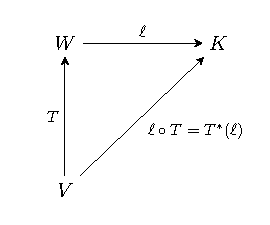
\includegraphics{doc/dual_map/dual_map.pdf}
		\caption{Map diagram of the dual map}
	\end{figure}
	We'll show now that $T^*$ is a linear map. Let $\ell \in W^*$, $\alpha \in K$. We have that $T^*(\alpha \ell) \in V^*$ is the map
	\begin{align*}
				T^*(\alpha \ell)(v) &= \big((\alpha \ell) \circ T\big)(v) = (\alpha \ell) (Tv) = \alpha \ell (Tv) = \alpha (\ell \circ T)(v) = \alpha \big(T^*(\ell)\big)(v)\\
				\Longrightarrow \qquad T^*(\alpha \ell) &= \alpha T^*(\ell).
	\end{align*}
	
	Now, let $\ell_1, \ell_2 \in W^*$. We have that $T^*(\ell_1 + \ell_2) \in V^*$ is the map
	\begin{align*}
		T^*(\ell_1 + \ell_2)(v) &= \big((\ell_1 + \ell_2) \circ T\big)(v) = (\ell_1 \circ T + \ell_2 \circ T)(v) = (\ell_1 \circ T)(v) + (\ell_2 \circ T)(v)\\
		&= \big(T^*(\ell_1)\big)(v) + \big(T^*(\ell_2)\big)(v) \\
		\Longrightarrow \qquad T^*(\ell_1 + \ell_2) &= T^*(\ell_1) + T^*(\ell_2).
	\end{align*}
	This shows that $T^*$ is linear as claimed. \qedhere
\end{proof}

\begin{proposition}{Composition of the Dual Map}{comp_dual_map}
	Let $U,V, W$ be vector spaces over $K$. Let $T:V \to W$, $S:W \to U$ be linear maps. Consider $T^*:W^* \to V^*$, $S^*:U^* \to W^*$, the dual maps. Then
	\[
		(S \circ T)^* = T^* \circ S^*.
	\]
\end{proposition}

\begin{lemma}{\textcolor{red}{Interpretation of the Matrix Transpose}}{int_mat_trans}
	Let $S:V \to W$ be a linear map between two finite dimensional vector spaces $V$ and $W$ over $K$. Let $\mathcal{B}$ be a basis for $V$ and $\mathcal{C}$ be a basis for $W$. Consider $S^*:W^* \to V^*$ and the bases $\mathcal{C}^*, \mathcal{B}^*$ for $W^*, V^*$ respectively. Then
	\[
		[S^*]^{\mathcal{C}^*}_{\mathcal{B}^*} = \big([S]^{\mathcal{B}}_{\mathcal{C}}\big)^T.
	\]
\end{lemma}

\begin{proof}
	Write $\mathcal{B} = (v_1, \hdots , v_n), \mathcal{C} = (w_1,\hdots , w_m)$. Define $A := [S]^{\mathcal{B}}_{\mathcal{C}}, A = (a_{ij})$. $A$ satisfies
	\[
		Sv_j = \sum_{i=1}^{m} a_{ij} w_i.
	\]
	Now, for $w_j^* \in \mathcal{C}^*$ we have by Lemma \ref{lem*dual_base}
	\begin{align*}
		S^*w_j^* &= w_j^* \circ S = \sum_{i=1}^{n} (w_j^* \circ S)(v_i) \cdot v_i^* = \sum_{i=1}^{n} w_j^*\big(S(v_i)\big)\cdot v_i^*\\
		&= \sum_{i=1}^{n}w_j^*\bigg(\sum_{k=1}^{m}a_{ki} w_k\bigg)\cdot v_i^* = 
		\sum_{i=1}^{n} \sum_{k=1}^{m} a_{ki} w_j^*(w_k) \cdot v_i^* =	\sum_{i=1}^{n} a_{ji} v_i^*.
	\end{align*}
	Therefore, the coordinates of $S^*w_j^*$ in the basis $\mathcal{B}^* = (v_1^*, \hdots , v_n^*)$ are
	\[
		\begin{pmatrix}
			a_{j1}\\
			\vdots \\
			a_{jn}
		\end{pmatrix},
	\]
	which is the row \#$j$ in $A$, represented as a column, or equivalently the column \#$j$ in the matrix $A^T$. \qedhere
\end{proof}

\subsection{Reflexitvity}
Let $V$ be a vector space over $K$. We have $V^*$, but also $V^{**} := (V^*)^*$ by applying 'dual' one more time, to $V^*$. $(V^*)^*$ is sometimes called the bidual space of $V$. Is there any relation between $(V^*)^*$ and $V$.

\begin{theorem}{The Canonical Isomorphism between $(V^*)^*$ and $V$}{canonic_iso_bidual}
	Let $v$ be a \textcolor{red}{finite} dimensional vector space over $K$. Then there exists a canonical isomorphism $\tau: V \to (V^*)^*$, given by
	\[
		\forall \, v \in V, \; \tau(v):V^* \to K
	\]
	is the map
	\[
		\tau(v)(\ell) := \ell(v) \quad \forall \, \ell \in V^*.
	\]
	In other words,
	\[
		V \owns v \overset{\tau}{\longmapsto} \big(V^*\owns \ell \longmapsto \ell(v) \in K\big).
	\]
\end{theorem}

\begin{remark}
	The map $\tau:V \to (V^*)^*$ exists and is defined in the same way as above regardless of $V$ being finite or infinite dimensional. Moreover, $\tau$ is always injective. However, when $V$ is infinite dimensional, $\tau$ fails to be surjective.
\end{remark}

\subsection{Naturality}
The map $\tau: V \to (V^*)^*$ exists for every space $V$, and is defined in the same way. To distinguish $\tau$'s for different spaces, denote it now by $\tau_V:V \to (V^*)^*$. Let $V, W$ be two vector spaces over $K$. Then for every linear map $T: V \to W$ we have
\begin{figure}[H]
	\centering
	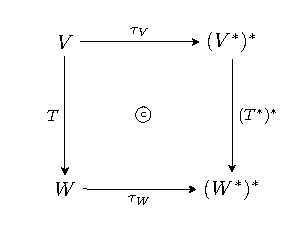
\includegraphics{doc/naturality/naturality.pdf}
\end{figure}
which we call naturality.

\begin{proposition}{Image of $\tau$}{img_tau}
	Let $V$ be a finite dimensional vector space over $K$, let $\mathcal{B} = (V_1,\hdots , v_n)$ be a basis for $V$. Let $\mathcal{B}^* = (v_1^*, \hdots , v_n^*)$ be the dual basis and $(\mathcal{B}^*)^* = ((v_1^*)^*,\hdots , (v_n^*)^*)$ the basis for $(V^*)^*$, which is dual to $\mathcal{B}^*$. Then $\tau(\mathcal{B}) = (\mathcal{B}^*)^*$, i.e.,
	\[
		\tau(v_i) = (v_i^*)^* \qquad \forall \, 1 \leq i \leq n.
	\]
\end{proposition}

\subsection{Direct Sums}

\begin{proposition}{The Vector Space of the Cartesian Product}
	Let $V, W$ be a vector space over $K$. Then the cartesian product $V \times W$ becomes a vector space over $K$ if we endow it with the following operations:
	\begin{itemize}
		\item[$\bullet$] $\forall \, (v_1, w_1), (v_2, w_2) \in V \times W : \; (v_1, w_1) + (v_2, w_2) := (v_1+v_2, w_1+ w_2)$.
		\item[$\bullet$] $\forall \, \alpha \in K, (v,w) \in V \times W : \; \alpha \cdot (v,w) := (\alpha v, \alpha w) \in V \times W$.
		\item[$\bullet$] $0_{V \times W} := (0_V, 0_W)$.
	\end{itemize}
	This new vector space $V \times W$ is usually denoted $V \oplus W$ and is called the direct sum of $V$ and $W$. We write the elements of $V \oplus W$ as $(v,w)$ or $v \oplus w$.
\end{proposition}

\begin{remark}
	$V \oplus W$ comes together with the following \textbf{canonical maps}:
	\begin{enumerate}
		\item[\textcolor{blue}{1)}] $i_V:V \to V \oplus W, \quad i_V(v) := (v,0)$.
		\item[\textcolor{blue}{2)}] $i_W:W \to V \oplus W, \quad i_W(w) := (0,w)$.
		\item[\textcolor{orange}{3)}] $p_V:V \oplus W \to V, \quad p_V(v,w) := v$.
		\item[\textcolor{orange}{4)}] $p_W:V \oplus W \to W, \quad p_W(v,w) := w$.
	\end{enumerate}
	The blue marked maps are canonical embeddings, while the orange marked maps are canonical projections.
	These maps are all linear. The maps $p_V, p_W$ are surjective, and $i_V, i_W$ are injective. Becuase of the maps $i_V, i_W$ we can sometimes view $V$ and $W$ as subspaces of $V \oplus W$.
\end{remark}

\begin{proposition}{The map $\varphi$}{map_phi}
	Let $V$ be a vector space over $K$, $U \subseteq V$ a subspace and $U' \subseteq V$ another subspace which is a complement of $U$ in $V$ (recall Definition \ref{def*lin_compl}). Then the map
	\[
		\varphi: U \oplus U' \to V, \quad \varphi(u, u') := u + u'
	\]
	is a linear isomorphism.
\end{proposition}

\begin{remark}
	When $U'$ is a complement of $U$ in $V$, then $U+ U' = V$ and we also have a canonical isomorphism $U \oplus U' \overset{\cong}{\longrightarrow} V$. But formally speaking $U \oplus U'$ is a different vector space than $V$.
\end{remark}

\subsubsection{Generalization to more Summands}
Let $U_1, \hdots , U_m$ be \textbf{finitely} many vector spaces over $K$. We can define $U_1 \oplus \hdots \oplus U_m := U_1 \times \hdots \times U_m$, with the coordinatewise/componentwise operations.

For \textbf{infinite} families $U_i,\, i\in \mathcal{I}$ one can define
\[
	\bigoplus_{i \in \mathcal{I}} U_i := \biggl\{t:\mathcal{I} \to \bigcup_{i \in \mathcal{I}} U_i \;|\; t(i) \in U_i \quad \forall \, i \in \mathcal{I}, \; t(i) \neq 0 \text{ for at most finitely many $i$'s}\biggr\}.
\]

\subsection{Quotient Spaces}
Let $V$ be a vector space over $K$, and $U \subseteq V$ a subspace. We will define a new vector space over $K$, $V/U$, together with a linear map $\pi :V \to V/U$ s.t. $\pi$ is surjective and $\ker(\pi) = U$. $V/U$ will have some other good properties. $V/U$ is called the \textbf{quotient of $V$ by $U$} or \textbf{$V$ modulo $U$}. $\pi$ is called the \textbf{quotient map} or the projection onto the quotient space.

We begin with an equivalence relation on $v$. Define for $v_1, v_2 \in V$
\[
	v_1 \sim v_2 \quad :\Longleftrightarrow \quad v_1 - v_2 \in U.
\]
We claim that $\sim$ defines an equivalence relation on $V$. Indeed
\begin{itemize}
	\item[$\bullet$]\textbf{Refelxivity:} $v \sim v$, b.c. $v - v = 0 \in U$.
	\item[$\bullet$]\textbf{Symmetry:} If $v_1 \sim v_2 \quad \Longrightarrow \quad v_2 \sim v_1$, b.c. $v_2 - v_1 = -(v_1 - v_2) \in U$.
	\item[$\bullet$]\textbf{Transitivity:} If $v_1 \sim v_2$ and $v_2 \sim v_3$, then $v_1 \sim v_3$, b.c. $v_1 - v_3 = \underbrace{(v_1 - v_2)}_{\displaystyle \in U} + \underbrace{(v_2 - v_3)}_{\displaystyle \in U} \in U$.
\end{itemize}
We denote the equivalence class of $v \in V$ by $[v]$. So
\[
	[v] = v + U = \{v + u \; |\; u \in U\},
\]
or equivalently
\[
	[v] = \{w \in V \; |\; v \sim w\} = \{w \in W\; |\; v - w \in U\}.
\]

\begin{definition}{Quotient Space}{quot_space}
	Let $V$ be a vector space over $K$ and $U \subseteq V$ a subspace. Define $V/U := V/\sim \, =$ the set of equivalence classes of the equivalence relation $\sim$. So, the elements of $V/U$ are $[v]$, where $v \in V$. Alternatively, each element in $V/U$ is a set of the form $v + U$, where $v \in V$. $V/U$ is called the \textbf{quotient of $V$ by $U$} (or modulo $U$).
\end{definition}

We want to turn $V/U$ into a vector space over $K$. To achieve this, we define:
\begin{itemize}
	\item[$\bullet$]\textbf{Addition:} $\forall \, [v_1], [v_2] \in V/U, \quad [v_1] + [v_2] := [v_1 + v_2] \in V/U$.
	\item[$\bullet$]\textbf{Mult. by a scalar:} $\forall \, \alpha \in K, [v] \in V/U, \quad \alpha \cdot [v] := [\alpha v] \in V/U$.
	(Alternatively written: $\alpha (v + U) := \alpha v + U$.)
	\item[$\bullet$]\textbf{The zero:} $0_{V/U} := [0_V]$. (Alternatively written: $0_{V/U} := 0_V + U$.) 
\end{itemize}

\begin{proposition}{Well Definedness of The Operations}{well_def_op}
	The operations above are well defined. Moreover, they give $V/U$ the structure of a vector space over $K$.
\end{proposition}

We now define the map
\[
	\pi:V \to V/U, \quad v \mapsto [v] \in V/U.
\]

\begin{proposition}{Properties of $\pi$}{prop_pi}
	$\pi$ is a linear map. Moreover, $\operatorname{Im}(\pi) = V/U$ (,i.e., $\pi$ is surjective), and $\ker(\pi) = U$.
\end{proposition}

\begin{proposition}{Dimension of $V/U$}{dim_quot_sp}
	Suppose that $V$ is finite dimensional. Then $V/U$ is finite dimensional too, and $\dim V/U = dim V - \dim U$.
\end{proposition}

\begin{theorem}{\textcolor{red}{The Isomorphism Theorem}}{iso_thm}
	Let $V, W$ be vector spaces over $K$ and $T: V \to W$ a linear map. Define a new map $\overline{T}:V/\ker(T) \to \operatorname{Im}(T)$, as follows. Let $x \in V/\ker(T)$. Choose a representative $v \in V$ for $x$, i.e., $x = [v]$. Define $\overline{T}(x) = \overline{T}([v]) := T(v)$. Then:
	\begin{enumerate}
		\item $\overline{T}$ is well defined, and is a linear map.
		\item $\overline{T}:V/\ker(T) \to \operatorname{Im}(T)$ is an isomorphism.
		\item The Diagramm in Figure \ref{fig:iso_thm} commutes, where $i:\operatorname{Im}(T) \to W$ is the inclusion.
	\end{enumerate}
	
\end{theorem}
\begin{figure}[h]
	\centering
	\label{fig:iso_thm}
	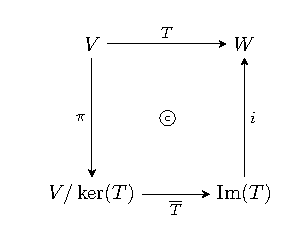
\includegraphics{doc/iso_thm/iso_thm.pdf}
	\caption{Map diagram of the map $\overline{T}$.}
\end{figure}

\begin{proof}
	\textbf{1) $\overline{T}$ is well defined:}. Suppose $x = [v] = [v'] \in V/\ker(T)$, we need to show that $T(v) = T(v')$. Indeed, $[v] = [v']$ implies that $v - v' \in \ker(T)$. Therefore, $T(v - v') = 0$. Since $T$ is linear we conclude that $T(v) = T(v')$.
	
	\textbf{$\overline{T}$ is linear:} Let $\alpha \in K, [v] \in V/\ker(T)$. By the linearity of $T$, the definition of the operations on the quotient space $V/\ker(T)$ and the definition of $\overline{T}$, we have that
	\[
		\overline{T}(\alpha [v]) = \overline{T}([\alpha v]) = T(\alpha v) = \alpha T(v) = \alpha \overline{T}([v]).
	\]
	Now, let $[v_1], [v_2] \in V/\ker(T)$. Then
	\[
		\overline{T}([v_1] + [v_2]) = \overline{T}([v_1 + v_2]) = T(v_1 + v_2) = T(v_1) + T(v_2) = \overline{T}([v_1]) + \overline{T}([v_2]).
	\]
	
	\textbf{2) $\overline{T}$ is injective:} Let $x \in \ker(\overline{T})$. Write $x$ as $x = [v]$ for some $v \in V$. Then
	\[
		\underbrace{\overline{T}(x)}_{\displaystyle = 0} = T(v).
	\]
	Therefore, $v \in \ker(T)$. Thus, $x = [v] = [0_V] = 0_{V/\ker(T)}$.
	
	\textbf{$\overline{T}$ is surjective:} Let $w \in \operatorname{Im}(T)$. Then there exists a $v \in V$ s.t. $T(v) = w$. Therefore, $\overline{T}([v]) = T(v) = w$. This shows that $\operatorname{Im}(T) \subseteq \operatorname{Im}(\overline{T})$.
	
	But by the definition of $\overline{T}$ we also have that $\operatorname{Im}(\overline{T}) \subseteq \operatorname{Im}(T)$.
	
	\textbf{3) The diagram commutes:} Let $v \in V$ and $w \in \operatorname{Im}(T) \subseteq W$ s.t. $T(v) = w$. Then by the definition of $\pi, \overline{T}$ and $i$, we have that
	\[
		(i \circ \overline{T} \circ \pi)(v) = (i \circ \overline{T})([v]) = i\big(T(v)\big) = i(w) = w.
	\]
	\qedhere
\end{proof}

\subsubsection{Universal Propertiy of Quotient Spaces}

\begin{theorem}{Universal Property of Quotient Spaces}{univ_prop_quot_space}
	Let $V$ be a vector space over $K$ and $U \subseteq V$ a subspace. The quotient space $V/U$ has the following universal property: 
	
	For every space $W$ and every linear map $T:V \to W$, for which $T(U) = 0$(, i.e., for which $U \subseteq \ker(T)$), there exists a \textbf{unique} linear map $T':V/U \to W$ s.t. the diagram in Figure \ref{fig:univ_prop} commutes. Moreover, $\ker(T') = \ker(T)/U$.
\end{theorem}
\begin{figure}[h]
	\centering
	\label{fig:univ_prop}
	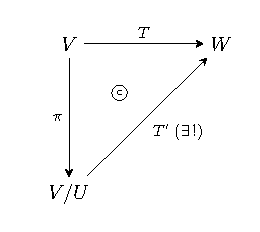
\includegraphics{doc/universal_property/universal_property.pdf}
	\caption{Map diagram of the map $T'$.}
\end{figure}

\textbf{Jargon:} Every linear map $T:V \to W$ that maps $U$ to 0 factors through $V/U$(, i.e., $T = T' \circ \pi$), and moreover in a unique way. We say that $T$ \textbf{induces} a map $T':V/U \to W$. We also say that $T$ \textbf{descends} to a map $T':V/U \to W$.

\subsubsection{Quotient Spaces \& Complements}

\begin{proposition}{A Canonical Isomorphism to a Complement}{canon_iso_compl}
	Let $V$ be a vector space over $K$ and $U \subseteq V$ a subspace. Let $W \subseteq V$ be a complement of $U$. Then there exists a canonical isomorphism $Q:W \overset{\cong}{\longrightarrow} V/U$, defined by
	\[
		Q(w) := [w] \in V/U \qquad \forall w \in W.
	\]
\end{proposition}

\begin{remark}
	The isomorphism $Q$ is canonical, only once $W$ is specified. In general there is no canonical choice of a complement $W$ to $U$. (In general there exist many choices of complements $W$ to $U$, and there is no preferred choice.)
\end{remark}

\subsection{Relations to Dual Spaces}

\begin{proposition}{Perpendicular Subspace}{purp_subsp}
	Let $V$ be a vector space over $K$ and $U \subseteq V$ a subspace. Define
	\[
		U^{\perp} := \bigl\{\ell \in V^* \;|\; \ell |_{U} = 0\bigr\},
	\]
	i.e., all the functionals on $V$ that vanish on $U$. Then:
	\begin{enumerate}
		\item $U^{\perp} \subseteq V^*$ is a linear subspace.
		\item There exists a \textbf{canonical} isomorphism $\big(V/U\big)^* \cong U^{\perp}$. If we assume that $V$ is finite dimensional then there exists a \textbf{canonical} isomorphism $U^* \cong V^*/U^{\perp}$.
	\end{enumerate}
\end{proposition}

\begin{proposition}{}{prop_perp_im}
	Let $T:V \to W$ be a linear map. Then
	\[
		(\operatorname{Im}(T))^{\perp} = \ker(T^*).
	\]
\end{proposition}




